\documentclass{article}
\usepackage{cite}
\usepackage{hyperref}
\usepackage{graphicx}
\usepackage{booktabs}
\usepackage{svg}

\title{A Graph-based Framework for Coverage Analysis in Autonomous Driving}
\author{Thomas Mühlenstädt and Marius Bause}
\date{\today}

\begin{document}

\maketitle

\section{Abstract}

test4

\section{Introduction}



In autonomous driving, coverage analysis is a crucial step to ensure the safety and reliability of the system.
In most situations, coverage arguments are collected either per coverage factor, or maybe up to 2 or 3 factor interactions.
See for example \cite{foretellix2019} for an production grade implementation of state of the art coverage analysis.
In contrast to existing approaches, this paper proposes a graph-based framework for coverage analysis.
There are already other graph-based approaches for analysing and representing traffic scenes.
However, the work in that paper is not specifically focused on coverage analysis.
Hence in this paper, graph based traffic scene representations are utilized for coverage analysis.

This paper is structured as follows: In chapter \ref{chapter:existing_approaches}, existing coverage and analysis approaches are discussed.
The basis for the following chapters is layed in chapter \ref{chapter:defining_a_traffic_scene_graph}. Afterwards, two coverage approaches 
using the traffic scene graphs are discussed in chapter \ref{chapter:create_subgraphs_for_coverage_analysis} and 
chapter \ref{chapter:implementation_of_graph_embeddings_for_traffic_scene_analysis}.
Finally, the developed methods are applied to Carla and Argoverse 2.0 data in chapter \ref{chapter:application} 
followed by a short summary and outlook.


\section{Existing coverage and analysis approaches}
\label{chapter:existing_approaches}

add Master thesis Johannes

There exist a larger 
The PEGASUS project (\cite{pegasus2019method}) introduces a systematic, scenario-based methodology for the verification and 
validation of highly automated driving functions, addressing the impracticality of traditional 
distance-based testing approaches. The core of the method is a six-layer model used to 
systematically describe and structure the driving environment, encompassing factors from road geometry to weather conditions. 
This framework is particularly relevant for coverage analysis, as it facilitates a structured decomposition of the vast, 
continuous test space into discrete, manageable "logical scenarios". By systematically 
parameterizing and exploring these logical scenarios across simulation, proving ground, and field tests, 
the methodology aims to ensure the completeness of relevant test runs and provides a structured 
foundation for arguing that the automated system has been adequately tested across its entire operational design 
domain (ODD). This shift from random sampling to a structured, scenario-based approach allows 
for a more efficient and comprehensive assessment to generate evidence for a final safety argumentation


The authors of (\cite{Ries2021traj_clustering}) address the challenge of validating automated driving systems 
in complex urban environments by proposing a trajectory-based clustering method for real-world driving data. 
They extract motion trajectories and associated features from urban driving recordings, apply unsupervised 
clustering to group similar driving behaviours/scenes, then analyze the resulting clusters to reveal common 
scenario types and redundancies. Their approach enables structuring the enormous scenario space, 
supporting more efficient test-set generation and scenario selection for automated vehicle verification. While 
not explicitly focused on coverage analysis, their approach is a good starting point for coverage analysis.


In \cite{Ulbrich2015scene}, the authors identify that key concepts in automated driving—namely scene, 
situation, and scenario—are inconsistently defined in the literature, which complicates the 
development, testing and validation of driving-automation modules. They propose clear 
definitions: a scene is a snapshot of the environment including dynamic and static 
elements plus actors’ self-representations; a situation is the set of all circumstances relevant for 
behaviour decision at a given moment, derived from the scene but reflecting the actor’s goals and 
values; and a scenario is a temporal development of several scenes in sequence, involving 
actions/events and goals/values. The paper also provides example implementations of these 
definitions in the context of automated-vehicle systems and how they interface with perception, 
planning and control, and testing.

Another important reference is the SAE International recommended practice \cite{ORAD2021taxonomy}, which 
provides many foundational terms in the context of autonomous driving.
It provides a functional taxonomy and clear definitions for key terms related to 
driving automation systems (DAS) used in on-road motor vehicles. The document defines six 
levels of driving automation (Levels 0 through 5) based on the role of three primary actors — 
the human driver, the driving automation system (DAS), and other vehicle systems/components. It introduces 
important related terms such as the Dynamic Driving Task (DDT), Operational Design 
Domain (ODD), Automated Driving System (ADS), and Vehicle Motion Control, 
among others. The 2021-04 revision (superseding the 2018 version) was developed in 
collaboration with ISO/TC 204/WG14 to harmonise global terminology and improve clarity for multi-discipline audiences 
(engineering, legal, media). The document emphasises that it is descriptive (not normative); 
it does not prescribe specifications or impose performance requirements for DAS.

The paper \cite{DBLP:journals/corr/abs-1801-08598} proposes a scenario-based framework for developing and 
validating automated-driving systems across different development phases. It 
introduces three abstraction levels of scenarios—functional, logical, and 
concrete—and discusses how these can be transformed for use in testing. The authors note that 
existing parameter-selection methods, such as equivalence-class or combinatorial testing, lack a 
systematic way to determine meaningful test coverage, highlighting coverage analysis as 
an open challenge in scenario-based validation.


In \cite{Ammann_Offutt_2008}, a standard textbook on software testing although not specifically focused on autonomous driving, the authors provide an 
introduction to software testing, which is a 
good starting point for coverage analysis. They introduce the concept of coverage and discuss the 
different types of coverage, such as statement coverage, branch coverage, condition coverage, 
and decision coverage. They also discuss the different techniques for measuring coverage, such as 
branch coverage, condition coverage, and decision coverage.

\cite{foretellix2019}

\cite{deGelder2022ontology}

\cite{wachenfeld2016release}



\cite{iso21448}

\cite{ul4600}


\section{Defining a traffic scene graph}
\label{chapter:defining_a_traffic_scene_graph}

still to be added: \url{https://sagroups.ieee.org/adwg/wp-content/uploads/sites/661/2024/10/ADWG_STV2_whitepaper.pdf}

still to be added: \url{https://www.vvm-projekt.de/securedl/sdl-eyJ0eXAiOiJKV1QiLCJhbGciOiJIUzI1NiJ9.eyJpYXQiOjE3NDc2OTIxNjgsImV4cCI6MTc0Nzc4MjE2OCwidXNlciI6MCwiZ3JvdXBzIjpbMCwtMV0sImZpbGUiOiJmaWxlYWRtaW4vdXNlcl91cGxvYWQvVlZNZXRob2Rlbl9adXNhbW1lbmZhc3NlbmRlcl9BYnNjaGx1c3NiZXJpY2h0X3YxLjBfenVyX1Zlc_f9d402f084002b57/VVMethoden_Zusammenfassender_Abschlussbericht_v1.0_zur_Veroeffentlichung.pdf}

\cite{newman2010networks}

\cite{bagschik2018ontologybasedscenecreation}



\cite{fremont2020scenic}


\subsection{time based graph representations}
The graph creation strategy described above is assuming to create a graph for a single timestep. One possible 
extension is to create a graph which contains information for multiple timesteps.

\begin{itemize}
    \item create a graph for multiple timesteps
    \item create a joint set of nodes. 
    \item For each time step, determine the corresponding edges.
    \item Add all edges to the graph, resulting in a di-graph, which can contain for a pair of nodes as many edges as there are time steps.
\end{itemize}

This extension allows the graph to easily represent changing states, e.g. the relationship between two vehicles 
changes from neighbor to leading vehicle, i.e. a cut in happened. One important special case for this type of processing is 
to handle actors, which are not present in all time steps, i.e. they appear and disappear during the time window. Especially 
if node attributes are used in the processing, a suitable imputation strategy is necessary to avoid 
non-equal dimensions of tensors for node attributes.

The methods derived in the following chapters can be applied to this extended graph representation as well, even though 
the focus in this paper will be on single timestep graphs.

\section{Analysing a traffic scene with a graph}

Having defined a graph-based traffic scene representation, we can now analyse the coverage of the system.
Two methodologies are proposed for this purpose:
One is to define archetypes of traffice scenes, and to compare graphs from observed traffic scenes to these archetypes.
The second one is to translate graphs to graph embeddings, and then to compare the embeddings of different sets of traffic scenes.

\section{Create subgraphs for coverage analysis}
\label{chapter:create_subgraphs_for_coverage_analysis}

There is a lot of knowledge in the literature on how to define archetypes of traffic scenes.
Once an archetype is defined, a special property of graphs can be used. 
Two graphs are isomorphic if they have the same structure, regardless of the node and edge labels.
As the archetypes are not necessarily are involving a lot of actors, these are more like subsets of actual traffic scenes.
A very simple example might be 2 vehicles on the same lane, driving in the same direction and another vehicle driving on a neighboring lane.
This situation can be represented by a graph with 3 nodes and 2 edges. 
In most real traffic situations however, there will be additional actors present, so that we are not searching for isomorphic graphs, but rather want to check if any subgraph of $G$ is isomorphic to the archetype graph $A$.
This is an example of a subgraph isomorphism problem.
While this problem is NP-hard, the graphs considered here are rather small, so the computational time is reasonable.
One such algorithm is the VF2 algorithm, which is implemented in the NetworkX library (see \cite{cordella2004subgraph}).
The strategy we are then applying is the following:

\begin{enumerate}
    \item Define a set of subgraphs $S$ that are considered to be archetypes of traffic scenes, e.g. unprotected left turns with opposite traffic or lead vehicle following situations.
    \item Define which node and edge attributes are considered for the isomorphism check.
    \item Create an empty dataframe $C$ with a column for each subgraph in $S$
    \item Define the set of traffice scenes (e.g. from Carla or Argoverse) defined as graphs $G$
    \item For each graph $G$, check if any subgraph of $G$ is isomorphic to any subgraph in $S$ and note the result in a new row in table $C$
\end{enumerate}



This strategy can be described to some degree as a bottom up approach: Starting from a detail level, individual situations are defined.
Then going upwards to different datasets, it is checked, if the archetype is present.
Also, follow up analysis of the created coverage dataframe can be performed. For example,

\begin{itemize}
    \item The distribution of numeric attributes like speed and and distance to other actors can be visualized for the subset of all traffic scenes which are subgraph isomorphic to an archetype.
    \item It can be cross tabulated, which combinations of archetypes are jointly present in a traffic scene.
    \item Pass Fail rates or other AV performance metrics can be calculated for the subset of all traffic scenes which are subgraph isomorphic to an archetype.
\end{itemize}

    

\section{Graph Embeddings for Traffic Scene Analysis}
\label{chapter:implementation_of_graph_embeddings_for_traffic_scene_analysis}

This section describes the concepts, implementation and application of graph embeddings to traffic scene graphs. 
The implementation follows a comprehensive approach to learning graph representations through self-supervised 
contrastive learning.

Embeddings are a widely used method to translate raw data like images or text into an embedding space in order to be 
able to perform machine learning tasks on them. One well known example of this is the Word2Vec model, which is used to 
translate words into a 
vector space, where the distance between vectors can be used to measure the similarity between 
words (\cite{mikolov2013efficientestimationwordrepresentations}).

In the context of traffic scene graphs, embeddings are used to translate the graph structure into a vector space, 
where the distance between vectors can be used to measure the similarity between traffic scenes.
This is useful for coverage analysis, as it allows to compare traffic scenes among each other.
For example, two traffic scenes can be considered similar if the distance between their embeddings is small. This enables
to search for a most similar simulation scenario given a real world scenario, to identify areas with near duplicates or 
to easily visualize structures in the embedding space, which in the original space of all possible traffic scenes
would not be possible.

Graph neural networks (GNNs) are a class of neural networks that are designed to process graph-structured data and have 
gained a lot of popularity in the last years, see for example (add references).

In this paper, a network architecture using a Graph Isomorphism Network with Edge features (GINE) as described 
in \cite{hu2020strategiespretraininggraphneural} is used to generate embeddings for traffic scene graphs as implemented in the 
pytorch geometric library (\cite{Fey/Lenssen/2019}). Main reason for using this specific architecture is that is capable of
learning embedding representations not only on the graph structure itself but on both node and edge attributes. Other 
network architectures like GraphSAGE or GAT are not capable of this. (TODO: check if this is true)

\begin{figure}[h]
    \centering
    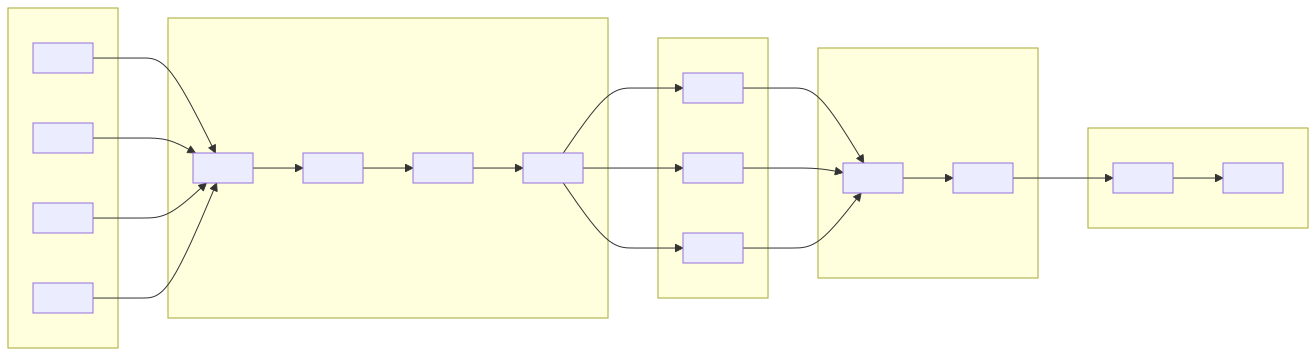
\includegraphics[width=0.8\textwidth]{plots/graph_gine_architecture.pdf}
    \caption{Model architecture for the Graph Isomorphism Network with Edge features (GINE).}
    \label{fig:graph_gine_architecture}
\end{figure}

The exact architecture of the model is shown in Figure \ref{fig:graph_gine_architecture}. The features 
used are the actor type (as a one hot encoding),
the actor speed (float), if the actor is on an intersection (boolean) and if the actor changed its 
lane since the last timestep (boolean) for the nodes.
For the edges, the edge type (as a one hot encoding) and the path length (float) between the two nodes are used.

The model has been trained on the CARLA and Argoverse 2.0 datasets using self-supervised contrastive learning. 


Training employed a self-supervised contrastive objective on mini-batches of 128 graphs. 
For each batch, two correlated views of every graph were created by 
perturbing continuous attributes with zero-mean Gaussian noise ($\sigma=0.1$) applied to node 
longitudinal speed and edge path length. A four-layer GINE encoder 
(hidden width 96) produced graph-level representations via the concatenation of 
mean, max, and sum pooling, followed by an embedding MLP (yielding 256-dimensional embeddings) and a projection head. The contrastive loss was a temperature-scaled cross-entropy over in-batch similarities (cosine similarity of $\ell_2$-normalized projections, temperature $\tau=0.1$), maximizing agreement of the two views of the same graph while contrasting against other graphs in the batch. Optimization used Adam with an exponentially decaying learning rate, initialized at 0.02 and multiplied by 0.75 across successive stages. 
This setup follows established practice in contrastive pretraining for GNNs \cite{hu2020strategiespretraininggraphneural} 
and is implemented using PyTorch Geometric \cite{Fey/Lenssen/2019}.


\begin{figure}[h]
\centering
\includegraphics[width=0.8\textwidth]{plots/train_test_graph_embeddings_loss_plot.png}
\caption{Training and test loss for the graph embeddings model trained jointly on CARLA and Argoverse 2.0 data.}
\label{fig:train_test_graph_embeddings_loss_plot}
\end{figure}


The resulting embeddings have been analysed in a number of ways. For plausibility checks, for a number of 
randomly samples scenarios, the scenario with 
closest embedding vector (euclidean distance as well as cosine distance) has been visualized. 
This is shown in Figure \ref{fig:plausibility_checks}. This 
includes comparison between CARLA and Argoverse scenarios.

\begin{figure}[h]
    \centering
    \includegraphics[width=0.8\textwidth]{plots/graph_embeddings_pca_tsne_test_plot.png}
    \caption{PCA and t-SNE visualization of the embedding space for Carla and Argoverse 2.0 scenarios.}
    \label{fig:embedding_space}
\end{figure}
    
As a next step, the embedding space has been analysed using PCA and t-SNE. This is shown in Figure \ref{fig:embedding_space}. This can be done in a number of 
different flavors, like for example:

\begin{itemize}
    \item distinguishing between CARLA and Argoverse scenarios by a color coding, 
    \item visualiizing just the CARLA scenarios and color code them by the map, in order to see if the maps deliver different types of scenarios,
    \item by calculating a density distribution of the embedding space for the Argoverse scenarios, and to check if for a regions with a density 
    about a certain threshold, there exist CARLA scenarios, i.e. do a coverage analysis in the embedded space
    \item do the same vice versa, i.e. to check for relevance of CARLA scenarios.
\end{itemize}

As the embedding space is a normal metric space, representing scenarios across a large range of different driving situations, these embeddings can be used also for 
many other tasks, like for example clustering, anomaly detection, similarity search, etc.

And, as the main task considered here is coverage analysis, the embeddings can be used to check if a target distribution is met by a test distribution in the embedded space. 
Specifically, considering the Argoverse 2.0 scenarios as the target distribution, and the CARLA scenarios as the test distribution, the embeddings can be used to check 
if the CARLA scenarios cover the Argoverse 2.0 scenarios in the embedded space.

The results for this approach are shown in Section xxx.


% The core component is the \texttt{TrainableGraphGINE} class, which implements a Graph Isomorphism Network with Edge features (GINE) architecture for generating graph-level embeddings. The model consists of multiple GINE convolutional layers, each containing:
% \begin{itemize}
%     \item Sequential multi-layer perceptrons (MLPs) with batch normalization and ReLU activations
%     \item Edge-aware message passing incorporating both node and edge features
%     \item Dropout regularization to prevent overfitting
% \end{itemize}

% The model employs a combination of three graph pooling strategies - mean, max, and sum pooling - to create a comprehensive graph-level representation. A projection head enables contrastive learning through InfoNCE loss, while an optional classification head supports supervised learning tasks.

% \subsection{Data Processing and Augmentation}

% The \texttt{GraphDataset} class handles the conversion from NetworkX graphs to PyTorch Geometric format through the \texttt{networkx\_to\_pyg} function. This conversion includes:
% \begin{itemize}
%     \item One-hot encoding of categorical node features (actor types: VEHICLE, PEDESTRIAN, CYCLIST, MOTORCYCLE)
%     \item One-hot encoding of edge types (neighbor\_vehicle, opposite\_vehicle, same\_lane, adjacent\_lane, following, intersection)
%     \item Preservation of continuous features such as longitudinal speed and path length
% \end{itemize}

% Data augmentation is implemented through the \texttt{augment\_graph} function, which adds Gaussian noise to continuous features to create augmented versions for contrastive learning.

% \subsection{Training Methodology}

% The training process utilizes self-supervised contrastive learning with the following characteristics:
% \begin{itemize}
%     \item InfoNCE contrastive loss implemented in the \texttt{contrastive\_loss} function
%     \item Adaptive learning rate schedule with exponential decay (starting at 0.02, decaying by factor 0.75)
%     \item Multi-epoch training with 15 epochs per learning rate stage
%     \item Data from both CARLA simulator (4,442 graphs) and Argoverse 2.0 dataset (3,588 graphs)
% \end{itemize}

% \subsection{Embedding Analysis and Visualization}

% The trained model generates 256-dimensional embeddings for each traffic scene graph. Analysis includes:
% \begin{itemize}
%     \item Dimensionality reduction using Principal Component Analysis (PCA) and t-distributed Stochastic Neighbor Embedding (t-SNE)
%     \item Visualization of embedding space distinguishing between CARLA and Argoverse data sources
%     \item Similarity-based scene retrieval using squared Euclidean distance in embedding space
%     \item Integration with visualization functions (\texttt{plot\_lane\_map\_advanced}, \texttt{add\_actors\_to\_map}, \texttt{add\_actor\_edges\_to\_map}) to display similar traffic scenes
% \end{itemize}

% The implementation demonstrates successful learning of traffic scene representations, with the embedding space capturing meaningful similarities between scenes from different data sources while maintaining distinction between simulation and real-world data.

\section{Application}
\label{chapter:application}

\subsection{Argoverse 2.0}

\cite{Argoverse2}

\subsection{Carla}

CARLA (Car Learning to Act, \cite{Dosovitskiy17Carla}) is an open-source simulator specifically designed for autonomous driving research and 
development. It provides a highly realistic urban driving environment with 
diverse road layouts, weather conditions, and traffic scenarios. The simulator features a comprehensive 
sensor suite simulation, flexible API for scenario creation, and supports both learning-based 
and traditional autonomous driving approaches. CARLA enables researchers to test and 
validate autonomous vehicle systems in a safe, controllable environment before real-world deployment.

The simulator has gained widespread adoption across both academic and industrial settings. In research, CARLA serves as a standard platform for developing and 
benchmarking autonomous driving algorithms, including reinforcement learning approaches for vehicle control and sensor fusion 
techniques \cite{codevilla2019exploringlimitationsbehaviorcloning}. Industry applications include 
virtual testing of production autonomous vehicle systems, scenario-based validation pipelines, and integration 
with hardware-in-the-loop testing frameworks \cite{jaeger2023hiddenbiasesendtoenddriving}. CARLA 
is also extensively used in autonomous driving competitions and challenges, providing a common evaluation 
environment for comparing different approaches across research groups worldwide.


Here, Carla version $0.9.15$ is used. The CARLA version $0.10.0$ is not used, because it had only 2 maps and
Mine\_1 (which is not really normal roads) at the start of this project.
Specifically, the following maps were used: Town01, Town02, Town03, Town04, Town05 and Town07. Plots
of these maps are shown in Figure \ref{fig:carla_maps}.

\begin{figure}[h]
\centering
\includegraphics[width=0.8\textwidth]{plots/carla_maps_used.png}
\caption{Overview of CARLA maps used in the simulation study: Town01, Town02, Town03, Town04, Town05, and Town07. These maps provide diverse urban driving environments with varying road layouts, intersections, and traffic patterns.}
\label{fig:carla_maps}
\end{figure}

The data generation script implements sophisticated behavior control mechanisms to create 
diverse and realistic traffic scenarios. Multiple vehicle types including trucks, motorcycles, 
and regular cars are spawned with varying probabilities, each exhibiting different behavioral
characteristics such as speed preferences, following distances, and lane-changing tendencies. 
The script incorporates dynamic behavior modifications during simulation, including random slowdowns, 
periodic behavior changes, and adaptive responses to traffic conditions, resulting in rich and 
varied traffic scene data across multiple CARLA maps and simulation iterations. The simulation runs
have between 20 and 60 vehicles each.

The resulting data consists of xxx scenes with 11 seconds of simulation time each, in order to have a 
similar data size as the Argoverse 2.0 dataset.

\begin{figure}[h]
    \centering
    \includegraphics[width=0.8\textwidth]{plots/subgraph_isomorphism_carla_coverage_barchart.png}
    \caption{Coverage barchart for the manually defined coverage scenarios for CARLA.}
    \label{fig:subgraph_isomorphism_carla_coverage_barchart}
\end{figure}

\begin{figure}[h]
    \centering
    \includegraphics[width=0.8\textwidth]{plots/subgraph_isomorphism_agreement_matrix_manual_scenarios_carla.png}
    \caption{Agreement matrix for manually defined coverage scenarios for CARLA.}
    \label{fig:subgraph_isomorphism_agreement_matrix_manual_scenarios_carla}
\end{figure}


\begin{table}[htbp]
    \caption{My Table}
    \label{tab:mytable}
    \begin{tabular}{rrrrr}
    \toprule
    scn 1 & scn 2 & scn 3 & scn 4 & size \\
    \midrule
    False & False & False & False & 613 \\
    False & False & True & False & 3 \\
    True & True & False & True & 377 \\
    True & True & True & True & 7 \\
    \bottomrule
    \end{tabular}
\end{table}
% \cite{goodfellow2016deep} % needed?

\begin{figure}[h]
    \centering
    \includegraphics[width=0.95\textwidth]{plots/combined_distributions_plots_speed_distance_carla.png}
    \caption{Agreement matrix for manually defined coverage scenarios for CARLA.}
    \label{fig:combined_distributions_plots_speed_distance_carla}
\end{figure}


\section{Summary}

\bibliographystyle{plain}
\bibliography{lit}

\begin{figure}[h]
    \centering
    \includegraphics[width=0.95\textwidth]{plots/graph_embeddings_comparison_plausibility_check_0.png}
    
    \includegraphics[width=0.95\textwidth]{plots/graph_embeddings_comparison_plausibility_check_1.png}
    
    \includegraphics[width=0.95\textwidth]{plots/graph_embeddings_comparison_plausibility_check_2.png}
    
    \includegraphics[width=0.95\textwidth]{plots/graph_embeddings_comparison_plausibility_check_3.png}
    
    \includegraphics[width=0.95\textwidth]{plots/graph_embeddings_comparison_plausibility_check_4.png}
    \caption{Plausibility checks showing graph embedding comparisons. For randomly sampled scenarios, the most similar scenarios based on embedding distance (both Euclidean and cosine) are visualized, including comparisons between CARLA and Argoverse scenarios.}
    \label{fig:plausibility_checks}
\end{figure}


\end{document}